\documentclass[aspectratio=169]{beamer}

% =============================================================
% PREAMBLE
% =============================================================

% --- PACKAGES ---
\usepackage[english]{babel}
\usepackage[T1]{fontenc}
\usepackage[utf8]{inputenc} 
\usepackage{graphicx}
\usepackage{booktabs} % For professional tables
\usepackage{tikz}     % For the pipeline diagram
\usetikzlibrary{shapes.geometric, arrows, positioning}
\usepackage{hyperref}

% --- CUSTOM BEAMER STYLE CONFIGURATION ---
% These must be defined BEFORE loading custom_beamer.sty

\def\true{1}
\def\false{2}

\def\colortheme{dark} % preset themes available are lighten, light, dark
\def\alertcolor{dark} % preset themes available are lighten, light, dark
\def\upperbar{\true} % i want upper index/navigation bar, \true or \false
\def\bottomsectionbar{\true} % i want bottom bar with Title and Frame/Slide number, \true or \false
\def\bottomtitlebar{\true} % i want bottom bar with Section and Institute, \true or \false

% Fix for alertblock colors
\usecolortheme{default}

% --- LOAD YOUR UNIVERSITY STYLE ---
\usepackage{custom_beamer}


% % %
\if\upperbar\false
    \setbeamertemplate{headline}{}
\fi
% % %

% --- METADATA ---
\title[Dense vs. Sparse Retrieval]{Reproducing ``Experimental Analysis of Dense vs. Sparse Retrieval''}
% \subtitle{An Experimental Analysis of Dense vs. Sparse Retrieval on the BEIR Benchmark}
\author{Gabriele Righi}
\institute{University of Pisa}
\date{\today}

% Link alla repository nel footer o nel titolo
\newcommand{\repoLink}{\url{https://github.com/Gheb6/dense-vs-sparse-retrieval}}

\begin{document}

% =============================================================
% SLIDE 1: Title Slide
% =============================================================
\firstpage

% =============================================================
% SLIDE 2: Introduction & Motivation
% =============================================================
\section{Introduction}

\begin{frame}{Introduction \& Motivation}
    \textbf{Context: Modern IR offers two main paths}
    \begin{itemize}
        \item \textbf{Sparse Retrieval:} BM25, SPLADE (Keyword-based, efficient).
        \item \textbf{Dense Retrieval:} Embeddings + ANN (Semantic-based, resource-heavy).
    \end{itemize}
    
    \vspace{1em}
    
    \textbf{The Problem}
    \begin{itemize}
        \item Dense retrieval is expensive (RAM/GPU). Is it always necessary?
    \end{itemize}
    
    \vspace{1em}
    
    \begin{alertblock}{Project Goal}
        Replicate the findings of \textit{Lin et al. (2024)} to answer:
        \begin{enumerate}
            \item Can \textbf{INT8 quantization} save memory without losing quality?
            \item Is \textbf{HNSW} (graph index) always better than \textbf{Flat} (brute-force)?
        \end{enumerate}
    \end{alertblock}
\end{frame}

% =============================================================
% SLIDE 3: Experimental Setup
% =============================================================
\section{Experimental Setup}

\begin{frame}{Experimental Setup}
    \begin{itemize}
        \item \textbf{Benchmark}: BEIR (Heterogeneous Evaluation).
        \item \textbf{Datasets Analyzed}: \texttt{scifact}, \texttt{nfcorpus}, \texttt{cqadupstack} (Android, Gaming, GIS).
        \item \textbf{Hardware}: NVIDIA T4 GPU (16GB VRAM).
        \begin{itemize}
            \item \textit{Constraints simulated a realistic production environment.}
        \end{itemize}
    \end{itemize}

    \vspace{1em}
    \textbf{Metrics}
    \begin{description}
        \item[nDCG@10] Retrieval Quality (Ranking accuracy).
        \item[Recall@10] Retrieval Coverage (Relevant items found).
        \item[QPS] Queries Per Second (Throughput/Speed).
    \end{description}
\end{frame}


% =============================================================
% --- NEW SLIDE 4: CHALLENGE 1 (Pyserini vs Faiss) ---
% =============================================================

\begin{frame}{Challenge I: The Missing Link in Pyserini}
    \textbf{Original Plan}: Use \texttt{Pyserini} (Lucene wrapper) for \textit{both} Sparse (BM25) and Dense (HNSW) indexing, matching the paper exactly.
    
    \vspace{1em}
    \textbf{The Obstacle}:
    \begin{itemize}
        \item Pyserini supports HNSW via Java, but the **Python API for adding vectors to HNSW indexes is limited/missing**.
        \item Impossible to feed custom BGE embeddings directly into Pyserini's HNSW from Python easily.
    \end{itemize}
    
    \vspace{1em}
    \textbf{The Engineering Solution: Hybrid Pipeline}
    \begin{itemize}
        \item \textbf{Sparse}: Kept Pyserini for BM25 (best-in-class implementation).
        \item \textbf{Dense}: Switched to \textbf{Faiss} (Facebook AI Search).
        \item \textit{Trade-off}: Faiss is C++/Python based (GPU friendly), diverging slightly from the paper's Lucene setup but enabling GPU acceleration.
    \end{itemize}
\end{frame}

% =============================================================
% SLIDE 4b: The SPLADE Anomaly (The Problem)
% =============================================================
\begin{frame}{Challenge II: The SPLADE Underperformance Mystery}
    \textbf{The Anomaly}
    While BM25 and Dense Retrieval matched the paper's baselines immediately, the standard SPLADE implementation (via Pyserini) failed.

    \begin{table}
        \centering
        \small
        \begin{tabular}{llcc}
            \toprule
            \textbf{Method} & \textbf{Implementation} & \textbf{nDCG@10} & \textbf{Status} \\
            \midrule
            BM25 & Pyserini (Lucene) & 0.323 & \textcolor{green!60!black}{\textbf{Success}} \\
            BGE Dense & Faiss & 0.370 & \textcolor{green!60!black}{\textbf{Success}} \\
            \textbf{SPLADE} & \textbf{Pyserini Impact} & \textbf{0.230} & \textcolor{red}{\textbf{Fail (-28\%)}} \\
            \bottomrule
        \end{tabular}
    \end{table}

    \vspace{0.5em}
    \textbf{Root Cause Analysis}
    \begin{itemize}
        \item \textit{Hypothesis A (Wrong Model)}: Switched to \texttt{selfdistil}. No change.
        \item \textit{Hypothesis B (Quantization)}: Forced integer scaling ($w \times 100$). No change.
        \item \textbf{Conclusion}: Pyserini's ``Black Box'' Impact Indexing was introducing \textbf{lossy compression artifacts}, destroying the precision of sparse weights.
    \end{itemize}
\end{frame}

% =============================================================
% SLIDE 4c: The Solution (Matrix Engine) - CONDENSED
% =============================================================
\begin{frame}{The Solution: Custom Matrix Engine}
    \textbf{The Fix}: Bypassed Pyserini. Built a \textbf{pure Python sparse engine} using \texttt{SciPy}.

    \vspace{1em}

    \begin{columns}
        \column{0.55\textwidth}
        \textbf{Methodology}
        \begin{itemize}
            \item \textbf{Direct Encoding}: Used HuggingFace to avoid quantization artifacts.
            \item \textbf{Vectorized Search}: Replaced index lookup with Matrix Multiplication.
        \end{itemize}
        
        \column{0.4\textwidth}
        \begin{block}{Core Logic}
            \centering
            \[ S = M_{docs} \times q^T \]
        \end{block}
    \end{columns}

    \vspace{1em}

    \begin{alertblock}{Impact}
        \begin{itemize}
            \item \textbf{Quality}: nDCG@10 restored to $\mathbf{0.357}$ (vs 0.230).
            \item \textbf{Speed}: $\sim$296 QPS (Efficient on Python).
        \end{itemize}
    \end{alertblock}
\end{frame}



% =============================================================
% SLIDE 5: Implementation Pipeline
% =============================================================
\section{Implementation}

\begin{frame}{Implementation Pipeline}
    % TikZ Diagram for the pipeline
    \begin{center}
    \resizebox{\textwidth}{!}{
        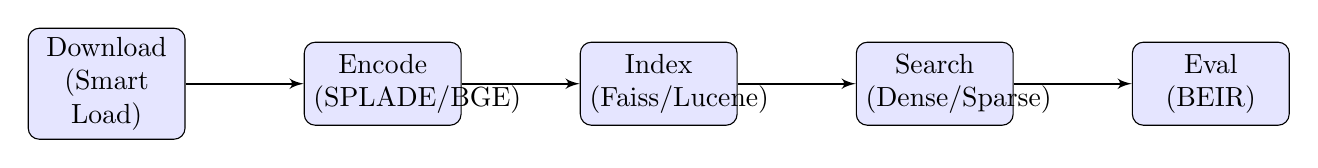
\begin{tikzpicture}[node distance=1.5cm, auto]
            \tikzstyle{block} = [rectangle, draw, fill=blue!10, text width=5em, text centered, rounded corners, minimum height=3em]
            \tikzstyle{line} = [draw, -latex', thick]
            
            \node [block] (dl) {Download (Smart Load)};
            \node [block, right=of dl] (enc) {Encode (SPLADE/BGE)};
            \node [block, right=of enc] (idx) {Index (Faiss/Lucene)};
            \node [block, right=of idx] (search) {Search (Dense/Sparse)};
            \node [block, right=of search] (eval) {Eval (BEIR)};
            
            \path [line] (dl) -- (enc);
            \path [line] (enc) -- (idx);
            \path [line] (idx) -- (search);
            \path [line] (search) -- (eval);
        \end{tikzpicture}
    }
    \end{center}

    \vspace{1em}
    \textbf{Key Contributions}
    \begin{itemize}
        \item \textbf{HuggingFace}: Efficient data loading (custom \texttt{Smart Loading} logic).
        \item \textbf{Pyserini (Lucene)}: Integration for BM25 indexing.
        \item \textbf{Faiss (GPU)}: Integration for Dense Retrieval (HNSW/Flat).
        \item \textbf{PyTorch}: Custom loop for SPLADE encoding.
    \end{itemize}
\end{frame}

% =============================================================
% SLIDE 7: Results - Quality (INT8 vs FP32)
% =============================================================
\section{Results}

\begin{frame}{Results - Quality (INT8 vs FP32)}
    % Example Table based on your Gaming data
    \begin{table}
        \centering
        \caption{Performance on \texttt{cqadupstack/gaming} (46k docs)}
        \begin{tabular}{lcccc}
            \toprule
            \textbf{Method} & \textbf{Quantization} & \textbf{nDCG@10} & \textbf{Recall@10} & \textbf{QPS} \\
            \midrule
            BGE-HNSW & FP32 & 0.587 & 0.726 & $\sim$467 \\
            BGE-HNSW & \textbf{INT8} & 0.584 & 0.723 & $\sim$519 \\
            \midrule
            BGE-Flat & FP32 & 0.587 & 0.726 & $\sim$1230 \\
            BGE-Flat & \textbf{INT8} & \textbf{0.584} & \textbf{0.724} & \textbf{$\sim$1212} \\
            \bottomrule
        \end{tabular}
    \end{table}

    \textbf{Findings:}
    \begin{itemize}
        \item nDCG drop is negligible (e.g., from 0.587 to 0.584).
        \item \textbf{Conclusion:} Quantization is ``operationally safe.'' It saves 75\% of memory with $<$0.5\% quality loss.
    \end{itemize}
\end{frame}

% =============================================================
% SLIDE 8: Results - Efficiency (HNSW vs Flat)
% =============================================================
\begin{frame}{Results - Efficiency (HNSW vs Flat)}
    \begin{columns}
        \column{0.5\textwidth}
        % PLACEHOLDER FOR YOUR PLOT
        % Replace 'example-image' with the path to your .pdf or .png file
        % E.g.: \includegraphics[width=\textwidth]{results/gaming_speed_vs_quality.pdf}
        \begin{block}{Speed vs Quality}
            \centering
            [Insert your scatter plot here]
        \end{block}

        \column{0.5\textwidth}
        \textbf{Surprising Result}
        \begin{itemize}
            \item On smaller datasets ($<$50k docs), \textbf{Flat Index outperformed HNSW} in QPS.
        \end{itemize}
        
        \vspace{1em}
        \textbf{Reasoning}
        \begin{itemize}
            \item HNSW suffers from random memory access patterns.
            \item Flat Index on GPU exploits massive parallelization.
        \end{itemize}
        
        \vspace{1em}
        \textbf{Takeaway}: HNSW is not a ``silver bullet.'' For specific vertical datasets, brute-force is faster.
    \end{columns}
\end{frame}

% =============================================================
% SLIDE 9: Code & Reproducibility
% =============================================================
\section{Reproducibility}

\begin{frame}{Code \& Reproducibility}
    The repository is organized to ensure full reproducibility:
    
    \vspace{1em}
    
    \begin{description}
        \item[\texttt{smart\_loading}] Efficient download logic (HuggingFace API).
        \item[\texttt{indexing}] Automated builders for Faiss (Dense) and Lucene (Sparse).
        \item[\texttt{evaluation}] Standardized BEIR metrics implementation.
    \end{description}
    
    \vspace{1em}
    
    \textbf{Robustness Features}
    \begin{itemize}
        \item Automatic detection of dataset schema variations (e.g., \texttt{query-id} vs \texttt{query\_id}).
        \item Universal download script for Colab and Kaggle environments.
    \end{itemize}
\end{frame}

% =============================================================
% SLIDE 10: Conclusions
% =============================================================
\section{Conclusions}

\begin{frame}{Conclusions}
    \textbf{Replication Successful:} Results align with the original paper's advice.
    
    \vspace{1em}
    
    \begin{block}{Operational Advice}
        \begin{enumerate}
            \item Use \textbf{INT8} by default for production (massive RAM savings, negligible quality loss).
            \item Use \textbf{Flat Index} for datasets $<$100k docs if a GPU is available (faster than HNSW).
        \end{enumerate}
    \end{block}
    
    \vspace{1em}
    \textbf{Future Work}
    \begin{itemize}
        \item Extend analysis to Binary Quantization (1-bit).
        \item Test on larger corpora (e.g., MS MARCO) to see the HNSW crossover point.
    \end{itemize}
\end{frame}

% =============================================================
% SLIDE 11: Q&A
% =============================================================
\begin{frame}
    \centering
    \Huge \textbf{Thank you!}
    
    \vspace{1em}
    \Large Questions?
    
    \vspace{2em}
    \normalsize
    \repoLink
\end{frame}

% =============================================================
% SLIDE 12: References
% =============================================================
\begin{frame}{References}
    \begin{thebibliography}{9}
        \bibitem{lin2024}
        S. Lin, S. Yang, and J. Lin,
        \textit{``Operational Advice for Dense and Sparse Retrievers: HNSW, Flat, or Inverted Indexes?''},
        arXiv:2409.06464, 2024.
        \newblock \url{https://arxiv.org/abs/2409.06464}
        
        \bibitem{repo}
        G. Righi,
        \textit{``Dense vs Sparse Retrieval - Replication Repository''},
        GitHub, 2026.
        \newblock \url{https://github.com/Gheb6/dense-vs-sparse-retrieval}
    \end{thebibliography}
\end{frame}

\end{document}

